\chapter{Material und Methoden}

Dieses Kapitel stellt die Deep-Learning-Architektur und das Dataset genauer vor, mit dem sich diese Thesis beschäftigt.
Grundlage der \glspl{can} sind die \glspl{gan}, weshalb diese zuerst betrachtet werden.
Anschließend erfolgt eine Erläuterung zur Architektur der \glspl{can} und welche Besonderheiten in Bezug auf die Segmentierung auftreten.
Zum Schluss wird das Datenmaterial vorgestellt, das in dieser Arbeit zum Einsatz kommt.



\section{Generative Adversarial Networks}

Maschinelles Lernen hat eine Klasse Algorithmen hervorgebracht, die sehr viele gelabelte Daten benötigen.
Um die Menge an benötigten Daten zu verringern, wird im Deep-Learning-Bereich an Ansätzen geforscht, die neue Trainingssamples generieren, fehlende Werte ausfüllen oder durch unüberwachtes Lernen oder Transfer Learning zu einer Verbesserung beitragen können~\cite{Goodfellow.2016}.
Viele dieser Entwicklungen basieren auf Modellen, die Wahrscheinlichkeitsverteilungen über die Trainingsdaten abschätzen, und solche Abschätzungen sind nur durchführbar, wenn man Inferenz approximiert.

Eine solche approximierte Inferenz bedingt eine Normalisierung über eine Konstante, deren Berechnung wiederum nur durch Approximation durchführbar wird.
Viele dieser Approximationen werden wegen der Abhängigkeit von allen Modellparametern mit wachsender Dimensionalität exponentiell schwieriger zu berechnen.
Häufig werden auf Markov-Ketten basierende Monte-Carlo-Methoden~\cite{Koller.2009} zur Berechnung der Normalisierungskonstante genutzt, aber diese funktionieren meist nur bei Konstellationen mit wenigen, nicht klar separierten Moden der Wahrscheinlichkeitsverteilung~\cite{Goodfellow.2016}.

Die \glspl{gan} von \citeauthor{Goodfellow.2014}~\cite{Goodfellow.2014} umgehen diese Herausforderungen durch die Gestaltung ihrer Architektur.
Ihr spieltheoretisch motivierter Ansatz, in dem zwei Netze gegeneinander arbeiten, ist mit Backpropagation trainierbar und benötigt somit weder approximierte Inferenz noch unkalkulierbare Normalisierungskonstanten.
Das Ziel ist es, möglichst realistisch wirkende Samples zu generieren.
\emph{Realistisch} bedeutet in diesem Kontext, dass ein erzeugtes Sample $ \mathbf{x} $ den Trainingsdaten sehr ähnlich, aber nicht identisch sein soll.

Das erste Netz, der \emph{Generator} $ G $, lernt eine Wahrscheinlichkeitsverteilung $ p_{\textup{data}}(\mathbf{x}) $ über die Trainingsdaten.
Aus einem zufällig initialisierten Vektor $ \mathbf{z} $ erzeugt er dann neue Samples.
Parallel dazu lernt das andere Netz, der \emph{Diskriminator} $ D $, immer besser zu beurteilen, ob ein Sample $ \mathbf{x} $ realistisch ist oder \emph{gefälscht}, also ob es aus den Trainingsdaten stammt oder vom Generator erzeugt wurde.

Der Generator versucht nun die Wahrscheinlichkeit zu maximieren, dass der Diskriminator einen Fehler macht und ein Sample falsch beurteilt~\cite{Goodfellow.2014}.
Als Zielfunktion ergibt sich

\begin{equation}\label{eq:gan}
\mathcal{L}(D, G) = \mathbb{E}_{\mathbf{x} \sim p_{\textup{data}}(\mathbf{x})} [\log D(\mathbf{x})] + \mathbb{E}_{\mathbf{z} \sim p_{\mathbf{z}}(\mathbf{z})} [\log(1 - D(G(\mathbf{z})))].
\end{equation}

Die eigentliche Verlustfunktion ist dann

\begin{equation}\label{eq:ganrisk}
R = \textup{arg}\min_G \max_D \mathcal{L}(D, G).
\end{equation}

Um Overfitting in $ D $ zu vermeiden, werden beide Netze von Grund auf trainiert, wobei bei jedem Trainingsschritt alterniert wird zwischen einem Update in $ D $ und einem Update in $ G $.
Es lässt sich zeigen, dass $ G $ auf diese Weise implizit eine Wahrscheinlichkeitsverteilung lernt, die den Trainingsdaten entspricht~\cite{Goodfellow.2014}.
Da $ D $ einen Skalar zwischen 0 und 1 ausgibt als Bewertung für die Realitätsnähe eines Samples, wird das Training als abgeschlossen betrachtet, wenn $ D $ für Samples aus den Trainingsdaten und generierte Samples den gleichen Wert ausgibt, nämlich $ \frac{1}{2} $.
In diesem Zielzustand kann der Diskriminator nicht mehr zwischen realen und gefälschten Samples unterscheiden; er kann dann verworfen werden.

Die visuelle Qualität der Erzeugnisse der originalen \glspl{gan} wurde in darauffolgenden Arbeiten deutlich verbessert.
Besonders die LAPGANs und \glspl{dcgan} haben sich hierbei hervorgetan.



\subsection{LAPGANs}

Die LAPGANs von \citeauthor{Denton.2015}~\cite{Denton.2015} basieren auf einer Laplace'schen Pyramide, bei der auf jeder Ebene ein gesondertes \gls{gan} eine Bildschärfung lernt.
Am Anfang erzeugt das erste \gls{gan} $ G_1 $ ein Sample mit sehr niedriger Auflösung, welches anschließend hochskaliert wird.
Das \gls{gan} der zweiten Ebene $ G_2 $ nimmt dann dieses hochskalierte, unscharfe Bild, und generiert dazu ein Restbild.
Dieses wird zum hochskalierten Bild addiert, das Ergebnis wird wieder hochskaliert und an die nächste Ebene weitergereicht, wo die nächste Schärfung stattfinden kann.
Der Prozess ist in \autoref{fig:lapgansampling} dargestellt.

\begin{figure}
	\centering
	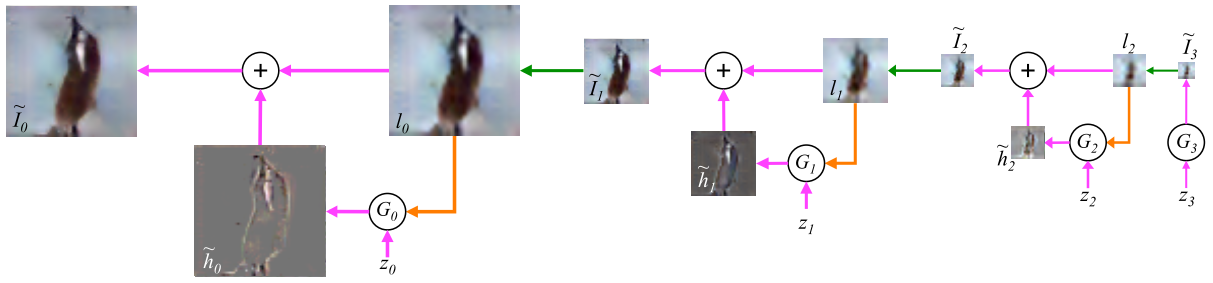
\includegraphics[width=0.9\linewidth]{img/lapgan_sampling}
	\caption{Sampling-Prozedur in LAPGANs (von rechts nach links)~\cite{Denton.2015}.}
	\label{fig:lapgansampling}
\end{figure}

Bis auf das erste \gls{gan} wird in diesem Fall auf jeder Ebene bereits eine konditionierte Variante der originalen \glspl{gan} verwendet.
Diese Modellvariante wurde schon bei \citeauthor{Goodfellow.2014}~\cite{Goodfellow.2014} vorgeschlagen und auch vor den LAPGANs bereits umgesetzt~\cite{Gauthier.2014,Mirza.2014}.
Im Kontext der konditionierten \glspl{gan} kommt eine konditionierende Variable $ \mathbf{y} $ hinzu, die sowohl an $ G $ als auch an $ D $ im Training und zur Inferenzzeit übergeben wird.
Dies erweitert die Zielfunktion von \autoref{eq:gan} zu

\begin{equation}\label{eq:canloss}
\begin{split}
\mathcal{L}_c(D, G) = & \ \mathbb{E}_{\mathbf{x}, \mathbf{y} \sim p_{\textup{data}}(\mathbf{x}, \mathbf{y})} [\log D(\mathbf{x}, \mathbf{y})] \\
+ & \ \mathbb{E}_{\mathbf{z} \sim p_{\mathbf{z}}(\mathbf{z}), \mathbf{x} \sim p_{\textup{data}}(\mathbf{x})} [\log(1 - D(\mathbf{x}, G(\mathbf{x}, \mathbf{z})))].
\end{split}
\end{equation}



\subsection{Deep Convolutional GANs}

Die \glspl{dcgan} von \citeauthor{Radford.2016}~\cite{Radford.2016} sind eine Weiterentwicklung der \glspl{gan}, deren Samples im Vergleich zu den LAPGANs weniger verrauscht sind.
Sie modifizieren die originalen \glspl{gan}, indem sie ähnlich den \glspl{fcn} nur noch Faltungsschichten statt Pooling- und vollständig verbundenen Schichten.
Außerdem nutzen sie in allen Schichten Batch-Normalisierung, was Mittelwert und Standardabweichung jedes Units einer Schicht auf respektive 0 und $ \pm 1 $ normiert.
Ebenso kommt als Aktivierungsfunktion im Generator nur noch das \gls{relu}~\cite{Nair.2010} und im Diskriminator das Leaky ReLU zum Einsatz; in der Ausgabeschicht des Generators erweist sich die Aktivierungsfunktion mit $ \tanh $ als erfolgreicher im Vergleich zu maxout bei den originalen \glspl{gan}.

Durch verschiedene Experimente können die Autoren zeigen, dass der latente Vektorraum, den das Modell lernt, tatsächlich glatte Übergänge hat, und dass die gelernten Filter zu häufig auftretenden Objekten korrespondieren.
Ebenso beobachten sie, dass das Unterdrücken von bestimmten Filtern dem Auslassen oder Transformieren bestimmter Objekte im generierten Sample entspricht, und dass simple Vektorarithmetik im latenten Vektorraum plausible Ergebnisse erzielt (s.~\autoref{fig:dcganarithmetic}).
All dies spricht dafür, dass diese Architektur nicht nur visuell ansprechende Ergebnisse erzielen kann, sondern auch eine stabile Repräsentation gelernt hat anstatt auswendig zu lernen und damit Overfitting zum Opfer zu fallen.

\begin{figure}
	\centering
	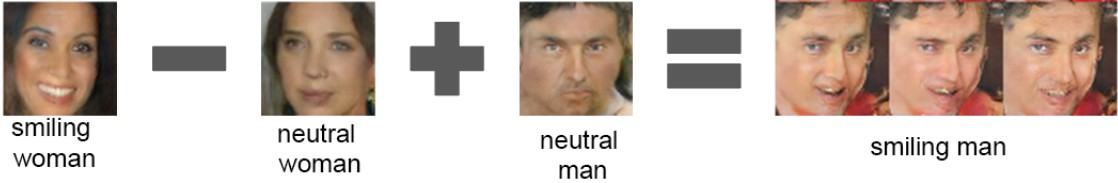
\includegraphics[width=0.9\linewidth]{img/dcgan_arithmetic}
	\caption{Beispiel für Vektorarithmetik in \glspl{dcgan}~\cite{Radford.2016}.}
	\label{fig:dcganarithmetic}
\end{figure}



\section{Conditional Adversarial Networks}

Die \glspl{can} von \citeauthor{Isola.2017}~\cite{Isola.2017} bestehen aus einem Generator und einem Diskriminator, die beide auf \glspl{dcgan} basieren.
Ihr Ansatz ist mit dem Zweck gestaltet, eine generische Architektur für Probleme bereitzustellen, bei denen eine Repräsentation eines Bildes auf eine andere Repräsentation eines Bildes abgebildet wird; die Autoren sprechen in diesem Zusammenhang von "Bild-zu-Bild-Übersetzung".

Im Gegensatz zu anderen Arbeiten, die konditionierte \glspl{gan} für spezielle Bild-zu-Bild-Probleme verwenden, ist in ihrer Architektur theoretisch \emph{nichts} anwendungsspezifisch angepasst.
Stattdessen ermöglicht es das GAN-Framework, dass die konkrete Verlustfunktion vollständig aus den Trainingsdaten gelernt wird, ohne dass diese problemspezifisch von Hand definiert werden muss.



\subsection{Generator}

Der Generator der \glspl{can} basiert auf dem \gls{dcgan}, muss aber in der konditionierten Variante erweitert werden, damit das Inputbild $ \mathbf{y} $ bei der Eingabe in den Generator herunterskaliert und dadurch enkodiert werden kann.
Man könnte dafür den Aufbau eines Encoder-Decoders wählen; tatsächlich orientiert sich der Generator konkret an der Struktur des U-Net~\cite{Ronneberger.2015}:
Diese Netzvariante ähnelt den \glspl{fcn}~\cite{Long.2015}, die bereits Skip Connections einbauen, damit trotz der Herunterskalierung Information aus den ursprünglichen Skalenstufen in die späteren Schichten des Netzes fließen kann.
Beim U-Net werden allerdings im Gegensatz zum FCN-8s nicht nur die niedrigsten drei Skalierungsstufen verbunden, sondern jede Schicht $ i $ wird mit der "gegenüberliegenden" Schicht $ n-i $ verbunden (s.~\autoref{fig:unetarchitecture}).
Zusätzlich entsprechen diese Skip Connections nicht der elementweisen Aufsummierung, sondern aus einem Anhängen der Kanäle von Schicht $ i $ an die Kanäle der späteren Schicht $ n-i $.

\begin{figure}
	\centering
	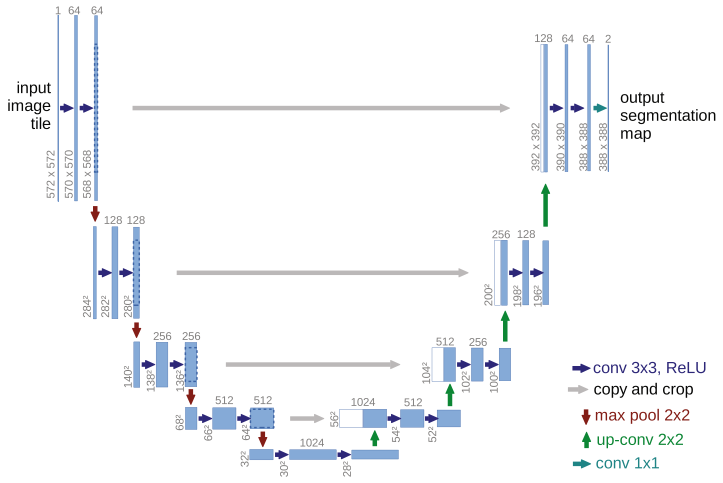
\includegraphics[width=0.7\linewidth]{img/unet_architecture}
	\caption{Architektur des U-Net~\cite{Ronneberger.2015}.}
	\label{fig:unetarchitecture}
\end{figure}



\subsection{Diskriminator}

Die Formulierung des Diskriminators in einem \gls{gan} entscheidet darüber, wie erfolgreich der Generator lernen kann, weil der Diskriminator ihm aufzeigt, welche Outputs realistisch wirken.
Damit der Diskriminator entscheiden kann, wie realistisch das Bild $ G(\mathbf{x}, \mathbf{y}) $ aussieht in Abhängigkeit vom Inputbild $ \mathbf{y} $, muss er ein Maß haben, um Bilder miteinander vergleichen zu können.
\citeauthor{Isola.2017} gestalten hier sowohl die Verlustfunktion als auch den Diskriminator ausgehend von der Hypothese, dass die niedrigen Frequenzen im Bild von herkömmlichen Distanzfunktionen sehr gut modelliert werden, aber die hohen Bildfrequenzen durch gelernte Funktionen abgedeckt werden müssen.

Verbreitete Maße zum Vergleich von Bildern sind die L1-Distanz mit $ \sum_i | \mathbf{x}_i - \mathbf{y}_i | $ und die L2-Distanz mit $ \sum_i (\mathbf{x}_i - \mathbf{y}_i)^2 $.
Solche pixelweisen Differenzen nehmen den Eingaberaum als unstrukturiert wahr.
Nutzt man ein solches Distanzmaß als Verlustfunktion in einem \gls{gan}, das Bilder generiert, kommen dabei meist nur unscharfe und graue Bilder heraus.
Scheinbar produziert der Einsatz dieser Maße eine unscharfe Ausgabe, wenn sie eine Bildkante nicht genau lokalisieren können, bzw. eine gemittelte graue Farbe, wenn sie eine auffällige Farbe nicht genau lokalisieren können~\cite{Isola.2017}.
Allerdings sind diese Maße in der Lage die groben Strukturen, also die tiefen Frequenzen im Bild, treffend abzubilden.
Deshalb kommt zur Einhaltung der Korrektheit in den tiefen Frequenzen die L1-Distanz in der Verlustfunktion zum Einsatz.

Der Diskriminator hingegen wird als \emph{PatchGAN} aufgebaut, der die feinen Strukturen und damit die hohen Frequenzen im Bild auf Realitätsnähe überprüfen kann.
(Der Name des Diskriminators ist irreführend gewählt, da es sich bei dem Diskriminator nicht um ein \gls{gan} handelt -- besser wäre vermutlich so etwas wie \emph{Patch-Diskriminator}.)
Dieser Diskriminator ist als Netzstruktur aufgebaut, die einen Filter mit fester Größe faltend auf dem gesamten Bild einsetzt.
Eine zu kleine Größe des Filters erzeugt Bilder, die kachelartige Artefakte aufweisen; ein Filter mit der vollen Bildgröße skaliert nicht gut für Bilder mit beliebiger Größe und liefert nicht so gute Ergebnisse wie ein Filter mit 70$\times$70 Pixeln.
Die Ausgabe des Diskriminators sind die Aktivierungen seiner letzten Schicht, was einer 30$\times$30-Matrix entspricht, wobei jedes Element dieser Matrix der Glaubwürdigkeit eines 70$\times$70-Ausschnitt des Bildes entspricht.

Diese Formulierung des Diskriminators drückt prinzipiell die gleiche Annahme wie die eines \gls{mrf} aus:
Ein Pixel ist nur von den Pixeln unabhängig, die von ihm durch einen gewissen Abstand getrennt sind.



\subsection{Verlustfunktion}

Die Verlustfunktion für konditionierte \glspl{gan} (s.~\autoref{eq:ganrisk}) wird bei den \glspl{can} von \citeauthor{Isola.2017} in zwei Punkten modifiziert:
Zum einen wird die im vorigen Abschnitt erwähnte L1-Distanz hinzugefügt, zum anderen wird der Rauschvektor ausgelassen.
Um die niedrigen Bildfrequenzen korrekt im \gls{can} zu modellieren, wird ein gewichteter L1-Term in der Verlustfunktion hinzugefügt:

\begin{equation}
R^* = \textup{arg}\min_G \max_D \mathcal{L}_c(D, G) + \lambda \mathcal{L}_{L1}(G)
\end{equation}

Die hohen Bildfrequenzen können dann durch die beiden Terme des Diskriminators im ersten Summanden abgedeckt werden (s. \autoref{eq:canloss}), die niedrigen Frequenzen werden durch den zweiten Summanden modelliert.
Die besten Ergebnisse über alle Bild-zu-Bild-Übersetzungsaufgaben wurde erzielt für $ \lambda = 100 $.

In der Zielfunktion der \glspl{gan} spielt der Rausch-Vektor $ \mathbf{z} $ als Startpunkt für $ G $ eine wichtige Rolle, damit der Generator überhaupt eine Ausgabe erzeugen kann.
Da der Generator allerdings bei den \glspl{can} bereits einen Input erhält, ist dieser nicht mehr notwendig und es ergibt sich folgende Formulierung der Zielfunktion:

\begin{equation}\label{eq:canlosswonoise}
\begin{split}
\mathcal{L}_c(D, G) = & \ \mathbb{E}_{\mathbf{x}, \mathbf{y} \sim p_{\textup{data}}(\mathbf{x}, \mathbf{y})} [\log D(\mathbf{x}, \mathbf{y})] \\
+ & \ \mathbb{E}_{\mathbf{x} \sim p_{\textup{data}}(\mathbf{x})} [\log(1 - D(\mathbf{x}, G(\mathbf{x})))].
\end{split}
\end{equation}

Rauschen wird zur besseren Stabilisierung des Trainings dennoch in Form von Dropout eingesetzt.

Die Autoren stellen zu Beginn ihres Ansatzes die Behauptung auf, dass die Verlustfunktion vollständig vom Netz gelernt wird und nicht für jedes Problem neu angepasst werden muss.
Dies ist nur insofern richtig, als dass die Probleme als Bild-zu-Bild-Übersetzung formuliert werden können.
Erstaunlich viele Aufgaben lassen sich als diese Klasse von Problemen betrachten, darunter Bildrekonstruktion aus Kantenbildern, Style-Transfer und Kolorierung von Graustufenbildern\footnote{Weitere Beispiele s. \url{https://phillipi.github.io/pix2pix/}}.
Auch semantische Segmentierung kann als ein solches Problem verstanden werden.



\subsection{Segmentierung}

Segmentierung wird in der Literatur klassischerweise definiert als

\begin{quote}Aufteilung des Bildes in mehrere verschiedene Regionen, wobei jede dieser Regionen gewisse Informationen oder Eigenschaften besitzt.~\cite[S.~29]{Ens.2011}\end{quote}

Im Fall der \emph{semantischen Segmentierung} sind diese Regionen \emph{Segmente} des Bildes, die Instanzen von bestimmten Objekten oder Gruppen solcher Objekte enthalten.
Bei einer Segmentierung mehrerer Klassen wird meist jedes Segment mit einer eigenen Farbe pixelgenau repräsentiert (s.~\autoref{fig:segnet_multiclassseg}), bei \emph{binären} Segmentierung mit nur einer zu segmentierenden Objektklasse wird meist ein Binärbild ausgegeben, wobei die Segmente weiß und der Hintergrund schwarz ist (s.~\autoref{fig:unet_binaryseg}).

\begin{figure}
	\centering
	\begin{subfigure}{.45\textwidth}
		\centering
		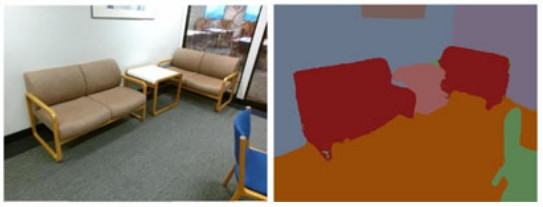
\includegraphics[width=0.9\linewidth]{img/segnet_multiclassseg}
		\caption{}
		\label{fig:segnet_multiclassseg}
	\end{subfigure}
	\begin{subfigure}{.45\textwidth}
		\centering
		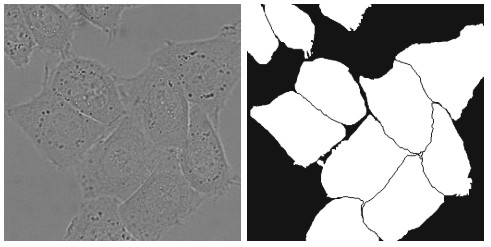
\includegraphics[width=0.9\linewidth]{img/unet_binaryseg}
		\caption{}
		\label{fig:unet_binaryseg}
	\end{subfigure}
	\caption{Beispiel von (a) Multiklassen-Segmentierung~\cite{Badrinarayanan.2017} und (b) binärer Segmentierung~\cite{Ronneberger.2015}.}
\end{figure}

\citeauthor{Isola.2017} überprüfen auch den Anwendungsfall einer semantischen Segmentierung mit einem Dataset von segmentierten Straßenszenen, wobei mehrere Objektklassen auftreten.
Die Kombination aus \gls{can} und L1-Distanz schneidet dabei schlechter ab als eine Verwendung von nur L1 als Verlustfunktion; letzteres liefert die besten Ergebnisse.
Scheinbar tendiert das \gls{can} dazu, übereifrig viele kleine Objekte zu segmentieren, die im Originalbild gar nicht vorkommen (s.~\autoref{fig:canseg}).

\begin{figure}
	\centering
	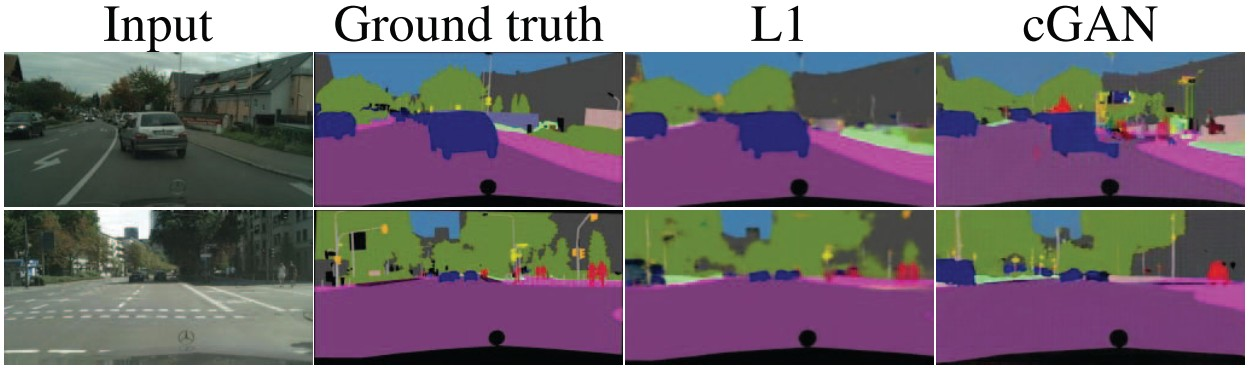
\includegraphics[width=0.9\linewidth]{img/can_seg}
	\caption{Ergebnisse von semantischer Multi-Klassen-Segmentierung bei \glspl{can}~\cite{Isola.2017}.}
	\label{fig:canseg}
\end{figure}

Zusätzlich produziert das \gls{can} keine vollständig diskreten Ergebnisse, bei denen die Segmentgrenzen klar sind, sondern tendenziell können auch Farbverläufe auftreten.
Allerdings wurde das \gls{can} noch nicht für eine binäre Segmentierung verwendet, was eben in dieser Arbeit getan wird.



\section{Form aus Sequenzbetrachtung}

Aus dem Stand der Technik und der Analyse von Koloskopie-Bildmaterial ergibt sich, dass neben sekundären Merkmalen wie Farbe und Textur die Form das aussagekräftigste Merkmal ist.
Aussagen über die Form würden wir am direktesten über die Tiefeninformation bekommen, aber wir haben oftmals nur monokulare Aufnahmen und damit keine unmittelbaren Tiefendaten vorliegen.
In der klassischen Bildverarbeitung ist es aber durch das Erfassen von Punktkorrespondenzen zwischen sequentiell aufgenommenen Bildern möglich, die Tiefeninformation einer Szene ungefähr zu rekonstruieren.
Dieser Bereich der Bildverarbeitung nennt sich "Structure from Motion".

Möglicherweise ist auch ein tiefes Netz dazu in der Lage, Tiefenstrukturen aus der Kamerabewegung abzuleiten.
Dazu muss man ihm allerdings mehrere konsekutive Frames zur Verfügung stellen.
Eine Architektur wie die 3D-FCNs liefert dafür eine gute Grundlage.

\subsection{3D-Faltung}

Den 3D-FCNs von \cite{Lequan.2017} liegen die 3D-CNNs zugrunde, welche zur Verarbeitung von dreidimensionalen Bilddaten genutzt werden können.
\citeauthor{Lequan.2017} nutzen diese allerdings unter der Annahme, dass ein Video auch nur ein 3D-Volumen ist.
Hierbei ist die zeitliche Komponente die dritte Dimension und die Zeitachse ihre Richtung -- es ergibt sich durch Aufeinanderstapeln der sequentiell angeordneten Frames ein 3D-Volumen.

[3D-Faltung erklären]

Bei den \glspl{can} ließe sich eine 3D-Faltung folgendermaßen umsetzen:
[]

\subsection{Optischer Fluss}

Zusätzlich zum 3D-Ansatz wäre auch eine reduzierte Variante mit optischem Fluss denkbar:
Man gibt dem Netz statt einem 3D-Volumen aus konsekutiven Frames einen einzelnen Frame inklusive der Information über den optischen Fluss vom vorherigen Frame zum jetzigen.
Je nach Geschwindigkeit des Tracking des optischen Flusses könnte dies die Gesamtperformanz des Systems theoretisch erhöhen, da maximal zwei Bilder auf einmal verarbeitet werden müssen.

Alle Teilansätze, die auf Seqenzbetrachtung beruhen, um Tiefeninformation zu generieren, sollten im Idealfall auch dann funktionieren, wenn nur ein einziger Input-Frame gegeben wird.

\subsection{Weitere DL-Methoden zur Tiefenschätzung}

\citeauthor{Mahmood.20171129} lassen mithilfe eines Transformer-GAN und Selbstregularisierung eine Transformation von realen zu synthetischen Bildern lernen, sodass dann auf dem synthetischen Bild die Tiefe geschätzt werden kann.
[sieht vielversprechend aus, aber steht uns nicht zur Verfügung]

\section{Dataset}

Im Zuge der MICCAI-Konferenz 2017 wurde auch eine neue Auflage der Endoscopic Vision Challenge ausgerichtet, die schon 2015 viele neue Ansätze in der endoskopischen Bildverarbeitung hervorbrachte.
Auch dieses Mal gab es wieder eine Sub-Challenge zur Polypen-Segmentierung, die Teil der GIANA ist.

[Herkunft der einzelnen Bestandteile des Datasets]

[Quantitative Beschreibung der Komponenten des Datasets]
